\documentclass[letterpaper,twoside]{article}
\usepackage{aistats2027}
\usepackage{amsmath,amssymb,amsthm}
\usepackage{booktabs}
\usepackage{graphicx}
\usepackage[round,authoryear]{natbib}
\renewcommand{\bibsection}{\subsubsection*{References}}
\usepackage{microtype}
\usepackage[hidelinks]{hyperref}
\hypersetup{
  pdftitle={Feature Normalization under Finite Training Budgets},
  pdfauthor={}
}

\newtheorem{theorem}{Theorem}[section]
\newtheorem{proposition}[theorem]{Proposition}
\newtheorem{lemma}[theorem]{Lemma}
\theoremstyle{remark}
\newtheorem{remark}[theorem]{Remark}
\DeclareMathOperator{\diag}{diag}
\DeclareMathOperator{\Cov}{Cov}
\DeclareMathOperator{\Var}{Var}
\DeclareMathOperator{\sign}{sign}
\newcommand{\E}{\mathbb{E}}
\newcommand{\Prob}{\mathbb{P}}
\newcommand{\R}{\mathbb{R}}
\newcommand{\soft}{S}

\begin{document}
\runningtitle{Feature Normalization under Finite Training Budgets}
\twocolumn[

\aistatstitle{Feature Normalization under Finite Training Budgets}

\aistatsauthor{Anonymous Authors}

\aistatsaddress{Anonymous Affiliations}
]

\begin{abstract}
  Feature normalization changes the relative rates at which stochastic gradient
  descent learns different coordinates. We study its consequences for prediction
  under finite training budgets, using common and rare binary features as a
  controlled setting. Exact error moments separate incomplete learning,
  randomness in feature sampling, and observation noise. For two independent
  features with known population preprocessing and one fresh observation per
  update, we prove opposite rare-subgroup risk orderings on two signal families.
  The gaps remain bounded away from zero as prevalence decreases, when the
  observation budget permits roughly one to four rare observations in
  expectation. Each normalization may choose any nonnegative constant learning
  rate and any deterministic stop within the budget. Scalar retuning therefore
  need not remove the prediction effect of relative feature scaling. Supporting
  comparisons show how stopping, batching, and dependence change specified
  procedures; both original anchor comparisons disappear after retuning.
  Existing experiments with estimated preprocessing and validation selection
  delimit practical conclusions. On a sparse categorical task, expanding the
  rate search removes a resolved standardization advantage under aggregate
  selection, while damped scaling retains lower risks. Missing rare validation
  cases can conceal severe subgroup errors. These experiments motivated the
  theory; a prospective evaluation of its predictions remains open.
\end{abstract}

\section{Introduction}

Feature normalization is part of the learning procedure. Dividing a predictor by
its standard deviation changes how quickly gradient methods learn its
coefficient and how strongly individual observations perturb that coefficient.
Under a finite training budget, these changes can affect the predictor even when
the unregularized least-squares solution is invariant to scaling. The
statistical question is therefore how normalization changes prediction at the
available budget, and which effects remain after calibrating the other training
choices.

Rare features make this question concrete. Without scaling, a rare binary
feature has small curvature and can remain poorly learned when common features
are already fitted. Standardization increases its learning rate relative to
common features. It also magnifies the stochastic contribution of the few
observations on which the feature is present. Early stopping and batch size
determine the balance between those effects. Dependence adds a further issue:
prediction for a rare subgroup depends on joint coefficient errors, so the
ordering of individual coefficient errors need not determine the ordering of
subgroup prediction risks.

We analyze squared-loss linear regression with a common and a rare binary
predictor. The population comparisons use known centering and scales, zero
initialization, a fixed intercept, and fresh observations at each update. Our
main result compares the lowest rare-presence risk attainable by each
normalization over all nonnegative constant learning rates and deterministic
stops within a common observation budget. Standardization wins on a specified
rare-signal family, and unscaled training wins on a common-signal family. Both
gaps are uniform as prevalence decreases with the expected number of rare
training observations held of order one. Thus relative scaling can change
attainable prediction risk even after separate scalar retuning. The theorem
concerns two independent features and one observation per update; it gives no
ordering over learning-rate schedules or data-dependent selection rules.

Supporting comparisons explain particular training paths. Standardization has
lower rare-presence risk at an early stop and higher risk later under a specified
rate calibration; a larger batch changes that ordering. Dependence can also make
aggregate and rare-presence risk favor opposite normalizations, even when
scaling increases both individual coefficient mean squared errors.

The existing experiments motivated the main theorem and examine the limits of
the supporting comparisons. A broader search over rates and stopping removes
both original anchor comparisons, although other laws retain reversals or
objective disagreements. Sampled-data experiments then
replace population preprocessing by estimated centering and scales, fit an
intercept, and select configurations on validation data. A sparse categorical
task shows a rare-subgroup benefit within the declared search, alongside
rate-boundary selections and a tradeoff with aggregate prediction. Missing rare
validation observations can conceal extreme subgroup error. These findings
motivate evaluating normalization as part of the full training and selection
procedure. They do not constitute a held-out test of the subsequently developed
oracle prediction.

\paragraph{Relation to prior work.}

The connection between preconditioning and statistical performance is
established \citep{amari2020preconditioning, su2024preconditioning}.
\citet[Section 4.2, Proposition 7]{amari2020preconditioning} relate preferred
preconditioning to signal alignment even after optimizing early-stopping bias
in an overparameterized fixed-data model. Our comparison concerns total
rare-subgroup risk, including stochastic-update variance, in a fixed-dimensional
fresh-sample model with an equal observation cap. It separates both complete
constant-rate and stopping families by explicit gaps. Early
stopping changes least-squares regularization \citep{ali2019early};
least-mean-squares analyses already separate bias and variance and study
sampling and batching \citep{defossez2015averaged, jain2018parallelizing}.
AdaBatch relates sparse mini-batch aggregation to coordinate rescaling
\citep{defossez2017adabatch}, and exact mean-square stability can be expressed
through moment operators \citep{mulayoff2024exact}. Target-aware preconditioning
under covariate shift also studies the dependence on the test objective
\citep{liu2025precondition}. For explicit regularization,
\citet{larsson2025normalization} analyze the influence of feature scaling on
shrinkage. Our comparisons specialize these broader mechanisms to conventional
normalization, final iterates, original-scale coefficients, and rare-presence
prediction. Neither diagonal preconditioning nor the existence of a
bias--variance tradeoff is a new mechanism here. The question is what
quantitative comparisons they yield, and how those comparisons change when the
entire training procedure is tuned.

\section{Normalization and the training procedure}
\label{sec:conference-setting}

Let $x$ be a centered feature vector with $C = \E[xx^\top] \succ 0$, and suppose
that $y = x^\top\beta^* + \varepsilon$, where $\E[\varepsilon\mid x] = 0$ and
$\E[\varepsilon^2\mid x] = \sigma^2$. We divide each feature by a positive scale
factor, collected in the diagonal matrix $S$. Training on $z = S^{-1}x$ with
parameter $\theta = S\beta$ then gives the following SGD update on the original
coefficient scale:
\begin{equation}
  \beta_{k+1}
  = \beta_k
    - \frac{\eta S^{-2}}{B} \sum_{i=1}^B x_{k,i}(x_{k,i}^\top\beta_k - y_{k,i}). \label{eq:conference-update}
\end{equation}
We use the average squared loss with a factor $1/2$. In the population
comparisons, we fix the centered intercept at zero and initialize $\beta_0 = 0$.
Each update uses $B$ independent fresh observations, so $k$ updates require
$M = kB$ observations. In Section~\ref{sec:conference-experiments}, we also
sample with replacement from a fixed training set of size $n$. There, $M$ counts
processed observations and can exceed $n$.

We can compensate exactly for global rescaling by adjusting the learning rate.
Replacing $S$ by $gS$ and $\eta$ by $g^2\eta$ leaves every update unchanged when
the methods use the same data stream. Changing the relative feature scales,
however, generally changes $\eta S^{-2}$ in a way that a single learning rate
cannot undo. Whether this leads to a risk difference after tuning requires a
separate comparison.

Write $e_k = \E[\beta_k-\beta^*]$ and
$V_k = \E[(\beta_k-\beta^*)(\beta_k-\beta^*)^\top]$. Fresh sampling gives
\begin{equation}
  V_k = e_ke_k^\top + A_k + \sigma^2N_k, \label{eq:conference-decomposition}
\end{equation}
where $A_k \succeq 0$ is the covariance of the noiseless process under random
feature sampling and $\sigma^2N_k \succeq 0$ is the covariance contributed by
observation noise. This decomposition separates incomplete learning from the two
sources of variation in training. We derive the exact recurrence in
Appendix~\ref{sec:comparison-proofs}.

For a subgroup $G$, we define the aggregate and subgroup excess prediction risks
using half squared loss:
\begin{equation}
  R_k = \tfrac12\operatorname{tr}(CV_k),\qquad R_{G,k}
      = \tfrac12\operatorname{tr}(C_GV_k), \label{eq:conference-risks}
\end{equation}
Here $C_G = \E[xx^\top\mid G]$ is the conditional second moment, which includes
the contribution of the conditional feature mean. Both risks exclude irreducible
test noise. We evaluate both objectives for the same trained predictor, without
changing the distribution of its training data.

\paragraph{Binary features.}

Let $I$ and $J$ be common and rare binary features, respectively, with
\[
  \begin{gathered}
    \Prob(I = 1) = \tfrac12,\qquad \Prob(J = 1) = q, \\
    \Prob(I = 1,J = 1) = \tfrac{q(1+\ell)}2,
  \end{gathered}
\]
where $0 < q < 1/2$ and $-1 \leq \ell \leq 1$. These ranges ensure that all four
cell probabilities are nonnegative. For $x = (I - 1/2,J - q)^\top$, write
$a = 1/4$, $b = q(1 - q)$, and $c = q\ell/2$. Then
\[
  C = \begin{pmatrix}
        a & c \\
        c & b
      \end{pmatrix},\qquad C_R
    = \begin{pmatrix}
        a             & \ell(1 - q)/2 \\
        \ell(1 - q)/2 & (1 - q)^2
      \end{pmatrix},
\]
where $R$ denotes the subgroup $J = 1$. A rare-coordinate error of one
contributes $(1 - q)^2/2$ to rare risk and $q(1 - q)/2$ to aggregate risk.

We compare unscaled features (U), with $P_U = I_2$, and standard-deviation
scaling (S), with $P_S = \diag(a^{-1},b^{-1})$, where $P = S^{-2}$. In the main
theorem, each rule chooses its own constant learning rate and stopping count.
For the supporting comparisons, we calibrate the rates through the common
coordinate. We use the final iterate in both settings.

\paragraph{Damped scaling.}

The sampled-data experiments also include damped scaling, with
\begin{equation}
  s_j = \sqrt{v_j + 0.01},\qquad P_{jj}
      = \frac{1}{v_j + 0.01}, \label{eq:conference-damped}
\end{equation}
where $v_j$ is either the known population variance or an estimate from the
training data. We use the heuristic offset $0.01$ from the controlled pilot,
fixed in variance units before evaluation. We neither derive this value from
theory nor select it by validation. At the same learning rate, damping
multiplies the SD update on the original coefficient scale by
$v_j/(v_j + 0.01)$. This is approximately one half at binary prevalence $0.01$
and $0.96$ for a balanced binary feature, illustrating how the offset reduces
updates more strongly for rare features. The comparison does not establish an
optimal damping level.

\section{Opposite risk orderings after oracle tuning}
\label{sec:conference-predictive}

We compare attainable rare-presence risk after separate scalar retuning for
independent features ($\ell = 0$), $B = 1$, and the population preprocessing,
zero initialization, and fixed intercept of
Section~\ref{sec:conference-setting}. Put $b = q(1-q)$. Parameterize the
original-coordinate update matrices by
\begin{equation}
 D_U(\alpha) = \alpha I_2,\qquad
 D_S(\alpha) = \diag(4b\alpha,\alpha),\quad \alpha\geq0.
 \label{eq:conference-oracle-rates}
\end{equation}
Here $D=\eta P$, so $\eta_U=\alpha$ and $\eta_S=b\alpha$. Each
parameterization covers every nonnegative constant learning rate for its rule.
The shared parameter is a coordinate for the search, not a constraint that the
selected rates match.

For an observation cap $M\in\mathbb N$, define
\begin{equation}
 R_A^*(M)=\inf_{\substack{\alpha\geq0\\ k\in\{0,\ldots,M\}}}
             R_{R,k}^{A}(\alpha),\qquad A\in\{U,S\}.
 \label{eq:conference-oracle-risk}
\end{equation}
Rates and stops are deterministic oracle choices, based on the population risk
averaged over training randomness. Initialization is eligible. The search
includes finite stops at rates that need not be mean-square stable.

\begin{theorem}[Opposite oracle rare-risk orderings]
 \label{thm:conference-predictive}
 Suppose $\sigma^2>0$, $0<q\leq10^{-4}$, and
 $1\leq Mq(1-q)\leq4$ in the independent binary model above.
 \begin{enumerate}
  \item If $(\beta_R^*)^2=\sigma^2$ and
        $(\beta_C^*)^2\leq\sigma^2/100$, then
        $R_U^*(M)-R_S^*(M)\geq7\sigma^2/1000$.
  \item If $(\beta_C^*)^2=\sigma^2$ and
        $(\beta_R^*)^2\leq\sigma^2/100$, then
        $R_S^*(M)-R_U^*(M)\geq\sigma^2/200$.
 \end{enumerate}
 Either sign is allowed for each coefficient. Both inequalities also hold if
 each rule searches only its mean-square-stable nonnegative constant rates,
 together with initialization.
\end{theorem}

The proof in Appendix~\ref{sec:predictive-proofs} bounds every rate and stop of
the losing rule and supplies one stable candidate for the winning rule. The
diagonal error moments obey an exact positive recurrence, even though stochastic
updates couple the independent features. For a dominant rare signal, learning
it with U also incurs common-coordinate noise; S can reduce that cost. For a
dominant common signal, S must balance incomplete common learning against rare
noise. U can learn the common coordinate while leaving the small rare signal
largely unchanged. The bounds establish strict orderings over whole families of
procedures without identifying their optimizers.

The expected rare training count at the cap is $Mq=\tau/(1-q)$, where
$\tau=Mq(1-q)\in[1,4]$. Thus the positive gaps concern a regime with roughly
one to four rare observations, even as $M$ grows and $q$ decreases. Prevalence
alone does not determine the preferred normalization. The two signal families
give sufficient conditions, without locating a general transition between them.
The theorem does not optimize batches, learning-rate schedules, or
data-dependent stopping, and supplies no guarantee for estimated preprocessing
or validation selection.

\section{Supporting comparisons under a fixed calibration}
\label{sec:conference-comparisons}

In this section, we fix $\eta_U = 4h$ and $\eta_S = h$. Both rules then have
diagonal drift $h$ in the common coordinate. Under independence, this gives the
common coefficient the same mean trajectory for both rules, although dependence
generally breaks the match. We specify $h$ in advance and use it for both
methods.

\subsection{Learning the rare signal versus fitting noise}

Under independence, SD scaling changes the contraction factor for the mean rare
coefficient error from $1 - 4hb$ to $1 - h$. At the same time, it increases the
observation-noise variance added to that coefficient at each update from
$16h^2b\sigma^2/B$ to $h^2\sigma^2/(bB)$. Standardization therefore speeds up
learning while introducing more noise. Random feature sampling contributes
additional variance to both procedures.

The diagonal error moments satisfy a nonnegative two-dimensional recurrence. By
omitting the terms that couple the two coordinates, we obtain a scalar
approximation to rare risk with an explicit nonnegative remainder. Let $F$ and
$N$ denote the noiseless and unit-noise parts of the SD-minus-U risk difference.
The approximation gives bounds
$F_- \leq F \leq F_+$ and $N_- \leq N \leq N_+$. When $F_+ < 0 < N_-$, the
noise-variance threshold $\tau = -F/N$ satisfies
\begin{equation}
 \frac{-F_+}{N_+} \leq \tau
                  \leq \frac{-F_-}{N_-}. \label{eq:conference-threshold}
\end{equation}
The remainder accounts for the dependence that the sampled updates introduce
between coefficient errors, even when the features are independent. We derive
the approximation and define its terms in Appendix~\ref{sec:comparison-proofs}.

\begin{theorem}[Stopping and batch reversal]
 \label{thm:conference-c1}
 In the binary model with $\ell = 0$, suppose
 \begin{gather*}
  q \in[0.019,0.021] ,\quad h \in[0.0019,0.0021] ,               \\
  \beta_C^*,\beta_R^* \in[0.95,1.05] ,\quad\sigma^2 \in[1.5,5] .
 \end{gather*}
 Both U and S are mean-square stable for $B \in \{1,10\}$. Their rare-risk
 contrast $\Delta_{B,k} = R_{R,k}^S - R_{R,k}^U$ lies in the intervals in
 Table~\ref{tab:conference-c1} throughout this parameter box.
\end{theorem}

\begin{table}[t]
 \centering
 \begin{tabular}{rrrr}
  \toprule
  $B$ &    $k$ & $M = kB$ &    $\Delta_{B,k}$ \\
  \midrule
    1 &  1,000 &    1,000 &   $[-.353,-.160]$ \\
    1 & 10,000 &   10,000 &    $[.0021,.125]$ \\
   10 &  1,000 &   10,000 &   $[-.386,-.286]$ \\
   10 & 10,000 &  100,000 & $[-.0281,-.0016]$ \\
  \bottomrule
 \end{tabular}
 \caption{
  Bounds on the rare-risk difference in Theorem~\ref{thm:conference-c1}, valid
  throughout the parameter box. Negative values favor SD scaling. The intervals
  enclose the exact risk differences and do not represent Monte Carlo
  uncertainty.
 }
 \label{tab:conference-c1}
\end{table}

At $B = 1$, the ordering reverses as training continues. With the same budget
$M = 10{,}000$, it also differs between $B = 1$ and $B = 10$. These are
comparisons between normalization rules at each batch size and budget. They do
not establish which batch size is better for either rule.

For the anchor $q = .02$, $h = .002$, $\beta^* = (1,1)^\top$, and
$\sigma^2 = 3$, the early $B = 1$ rare risk is $.356678$ for U and $.090407$ for
S. Squared bias contributes $.353207$ and $.011040$, respectively, so the early
advantage comes mainly from learning the rare signal more quickly. By
$k = 10{,}000$, U has learned enough of that signal to reach risk $.028145$,
whereas S has risk $.078788$, almost entirely due to observation noise. The
exact calculation includes variation from feature sampling at every step.

\subsection{Aggregate and rare-presence objectives}

Dependence can make the two prediction objectives favor different rules. Let
$\Delta V = V_k^S - V_k^U$. Direct substitution into \eqref{eq:conference-risks}
gives
\begin{equation}
 \Delta_R - \Delta_A = \frac{1 - 2q}{2}\bigl\{(1 - q)\Delta V_{RR} + \ell\Delta V_{CR}\bigr\}, \label{eq:conference-objectives}
\end{equation}
where $\Delta_A$ and $\Delta_R$ denote the aggregate and rare-risk differences.
The cross moment is the sum of the product of the coefficient biases and the
covariance of their errors.

\begin{theorem}[Objective disagreement]
 \label{thm:conference-c2}
 Take $q = .02$, $\ell \in[.9,1]$, $\beta^* = (2,1)^\top$, $h = .01$, $B = 1$,
 $k = M = 100$, and $\sigma^2 \in[3.8,4.1]$. Both U and S are mean-square
 stable, and uniformly over these intervals,
 \begin{align*}
  .00077 & \leq R_k^S - R_k^U \leq .00194,         \\
  -.0983 & \leq R_{R,k}^S - R_{R,k}^U \leq -.0233.
 \end{align*}
 Moreover, $V_{CC,k}^S > V_{CC,k}^U$ and $V_{RR,k}^S > V_{RR,k}^U$.
\end{theorem}

SD scaling increases each coefficient's mean squared error but improves
rare-presence prediction. At $\ell = 1$ and $\sigma^2 = 4$,
\[
 \Delta V \approx \begin{pmatrix}
                   .022743  & -.615146 \\
                   -.615146 & .470335
                  \end{pmatrix}.
\]
The reduction in the cross moment offsets the larger individual errors when
predicting for the rare subgroup. Aggregate risk gives this moment weight
$.01$, whereas rare risk gives it weight $.49$. Looking only at the individual
coefficient errors would therefore miss the improvement in rare prediction.

We prove both theorems using rational interval arithmetic with outward rounding
over the full parameter boxes. Appendix~\ref{sec:comparison-proofs} gives the
recurrences and enclosure arguments. The results apply to the specified
training procedures, whereas Theorem~\ref{thm:conference-predictive} compares
risks after optimizing over all constant rates and deterministic stops. Adaptive
stopping and the choice of an optimal normalization remain outside these
results. The identity relating the two risk objectives is elementary.

\section{From calibrated comparisons to selected procedures}
\label{sec:conference-experiments}

The experiments ask which effects remain when we change the comparison
protocol. We distinguish three settings: exact fresh-sample moments,
replacement SGD on sampled noisy training sets, and held-out evaluation
on a fixed categorical dataset. An observation budget counts every sampled
training row, including repeated visits. All results below concern final
iterates selected from stored checkpoints.

\subsection{Rate and stopping adjustments}

A follow-up exact-moment study covers 228 binary laws, 51,048 training
configurations, and 2,571,800 endpoints. It varies prevalence, dependence,
signal, noise, rates, batches, and stopping, and retains fixed-update and
fixed-observation comparisons. The primary adjusted comparison selects
the lowest exact risk among mean-square stable configurations and
initialization. It uses a coarse rate range from $1.953125\times10^{-6}$
to $.64$, with a separate resolution check on 16 laws. This is oracle
selection with a known test law, not validation selection.

Both original anchor comparisons disappear after the declared adjustments.
For the independent anchor of Theorem~\ref{thm:conference-c1},
Table~\ref{tab:conference-adjustment} reports the rare-risk gap at the
fixed configuration and after rate/stopping selection. The late $B=1$
disadvantage for S disappears; the selected rates are $h_U=.004$ and
$h_S=.0003125$. At the dependent anchor of
Theorem~\ref{thm:conference-c2}, adjusted selection favors U under both
objectives. Other laws retain reversals or produce objective disagreement.
The theorems therefore describe a calibrated procedure, while the search
answers a different question about the available family of procedures.

\begin{table}[t]
\centering
\begin{tabular}{rrrr}
\toprule
$B$ & $k$ (cap) & Fixed gap & Adjusted gap \\
\midrule
1 & 1,000 & $-.266270$ & $-.005695$ \\
1 & 10,000 & $+.050643$ & $-.002562$ \\
10 & 1,000 & $-.334899$ & $-.001381$ \\
10 & 10,000 & $-.014046$ & $-.000103$ \\
\bottomrule
\end{tabular}
\caption{SD-minus-U rare risk at the independent anchor. Adjusted gaps
use the declared coarse stable oracle search at the same observation cap.
The original stopping reversal disappears under this search.}
\label{tab:conference-adjustment}
\end{table}

The study retains invalid candidates in unrestricted reports rather than
silently removing them. Some unrestricted comparisons remain unresolved
because of overflow or invalid moment calculations. A paired Monte Carlo
covariance diagnostic also exceeds its declared gate in one tail-dominated
case; a conditional-absence investigation is retained with that result.
Neither issue is converted into a claim of complete simulation agreement.
The exact stable comparisons and these diagnostic limits have separate
roles in the evidence.

\subsection{Estimated preprocessing and validation selection}

The sampled-data stage uses eight binary laws, 128 independent replications
per law, $n=256$ training observations, and 128 validation observations.
It compares known preprocessing, estimated scales, training centering with
a fixed or fitted intercept, and an uncentered fitted-intercept arm.
The feature divisors are $1$, $\sqrt{v_j}$, and $\sqrt{v_j+.01}$, with
training variances using denominator $n$. Constant training columns are
frozen at zero coefficient with divisor one. Fitted intercepts start at
the training response mean. Appendix~\ref{sec:practical} gives further
protocol details.

Each scaling and preprocessing arm receives the same five rate factors
\[
 \eta=\frac{a_0}{\max(L,10^{-12})},\qquad
 a_0\in\{.001,.01,.05,.2,.8\},
\]
where $L$ is the largest empirical curvature, including the intercept
coordinate when fitted. This calibration does not guarantee stochastic
stability. Batches are $B\in\{1,16\}$ and observation caps are
$M\in\{128,512,2048\}$. We compare fixed $a_0=.05$, $B=16$ with
validation selection of rate and batch, or rate, batch, and stopping.
Initialization is eligible. Ten paths per arm and scaling cost $10M$
processed observations at cap $M$; checkpoints share paths. Selection
never uses test outcomes, and selected models are not refitted.

For the independent equal-signal law at $q=.02$ and $\sigma^2=3$,
the centered, fitted-intercept arm has fixed-configuration rare-risk gaps
of $-.1653$ (paired MCSE $.0295$) at $M=128$ and $+.0901$ ($.0697$)
at $M=2048$. The early advantage is clear; the late disadvantage is within
two MCSE of zero. At the latter budget, the rare-only signal favors S by
$.2320$ ($.0233$), while the common-only signal favors U by $.1272$
($.0159$). These sampled-data results use empirical rate calibration,
so they do not extend the exact population theorems.
Figure~\ref{fig:conference-practical} shows the fixed paths and the
categorical-task comparisons described below.

\begin{figure*}[t]
\centering
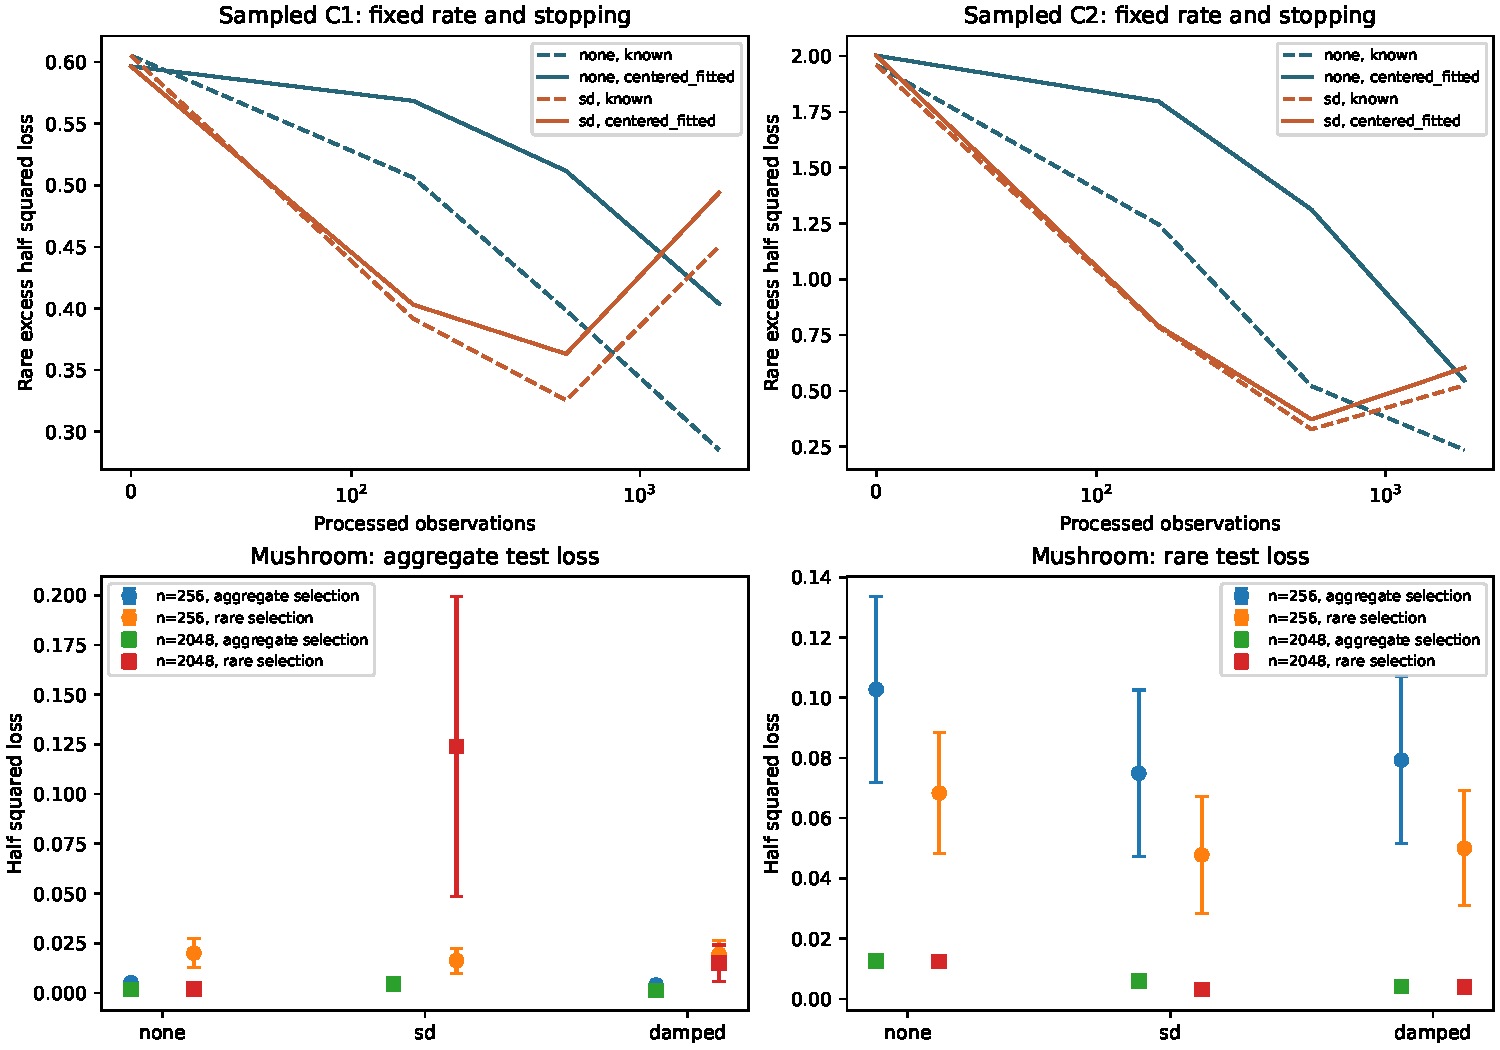
\includegraphics[width=\textwidth]{../results/practical-selection/practical-selection.pdf}
\caption{Practical normalization comparisons from the frozen sampled-data
study. Top: fixed-configuration paths for the independent and dependent
anchor laws under known preprocessing and training centering with a fitted
intercept. These use empirical rate calibration, not the theorems' fixed
$h$. Bottom: Mushroom held-out risks under aggregate and rare validation
selection at both sample sizes. Error bars show one Monte Carlo standard
error across replications or partitions; they are not population confidence
intervals for the Mushroom source.}
\label{fig:conference-practical}
\end{figure*}

\paragraph{When validation contains no rare cases.}
At $q=.002$, the two anchor laws have empty rare validation groups in
106 and 105 of 128 replications. The declared rare-selection rule falls
back to aggregate loss in those cases. One selected centered SD fit has
rare coefficient about $-6.719\times10^{16}$ and validation half squared
loss $2.086$, but exact-cell rare loss about $2.257\times10^{33}$.
A 160-digit decimal replay of all eligible trajectories in the worst
selected replication of each of 24 law/scaling panels leaves all 24
selections unchanged. The failure is not explained by detected
floating-point cancellation. Extreme finite outcomes and 151 failed
synthetic endpoints remain in the archive; tail-dominated means are not
precise population-risk estimates.

\subsection{A sparse categorical prediction task}

We predict the recorded poisonous label in UCI Mushroom
\citep{uciMushroom} using squared loss and all 22 categorical predictors.
The declared subgroup is green spore-print color: 72 of 8124 records.
Training data alone determine the one-hot vocabulary, means, and scales.
Missingness is a category and unknown categories map to zero blocks.
The design uses sparse storage and algebraic centering. Coefficients are
reported on the original feature scale; in the rank-deficient full
one-hot design, they are optimizer-dependent rather than uniquely
identified effects. Predictions are not clipped.

We use 32 random partitions at each training/validation size $(256,128)$
and $(2048,1024)$, with remaining records reserved for testing. Candidates
share partitions and replacement index streams. Each scaling receives the
same five rate factors and $B\in\{16,128\}$, with
$M\in\{512,2048,8192\}$. Table~\ref{tab:conference-mushroom} reports the
largest sample and cap with joint rate, batch, and stopping selection.

\begin{table}[t]
\centering
\begin{tabular}{llrr}
\toprule
Selection & Scaling & Aggregate & Rare \\
\midrule
Aggregate & None & .001754 & .012482 \\
 & SD & .004617 & .005912 \\
 & Damped & .001175 & .004151 \\
Rare & None & .001878 & .012465 \\
 & SD & .123905 & .003158 \\
 & Damped & .014966 & .003984 \\
\bottomrule
\end{tabular}
\caption{Mean held-out half squared loss for Mushroom, with $n=2048$,
1024 validation records, a fitted intercept, and cap $M=8192$.
Each scaling receives ten trajectories. Paired uncertainty is reported
in the text; marginal MCSEs appear in Appendix~\ref{sec:practical}.}
\label{tab:conference-mushroom}
\end{table}

Under aggregate selection, the SD-minus-none rare gap is $-.00657$
(paired MCSE $.00153$), with aggregate gap $+.002863$ ($.00213$).
Selecting SD by rare loss instead reduces its rare loss by $.002754$
($.000967$), with a variable aggregate penalty of $.11929$ ($.0756$).
The mean green coefficient under aggregate selection is $.4822$ for
none, $.7462$ for SD, and $.7678$ for damped scaling. Other coefficients
partly offset this larger contribution to rare predictions.

The result is conditional on the declared search. All 32 large-sample
unscaled aggregate selections choose the largest rate factor, so its
continuous optimum is unresolved. The small-sample experiment has no
green training observations in five partitions and none in validation
in thirteen. MCSEs describe partition and optimization variation within
this dataset. The source comprises hypothetical descriptions derived
from a field guide, so random-record performance does not establish
generalization to new species or field data.

\section{Discussion}

Feature normalization changes how quickly a model learns different coefficients
under a finite training budget. We have shown that this can affect the best
attainable rare-subgroup risk even when each method may choose any nonnegative
constant learning rate and any deterministic stop within the budget.
Standardization has lower risk on the specified rare-signal family, whereas
unscaled training has lower risk on the common-signal family. The gaps remain
bounded away from zero as prevalence decreases while the expected number of
rare observations stays of order one. The theorem thus gives sufficient
conditions for both orderings, although it does not locate a general boundary
between them.

The supporting comparisons explain how standardization can reduce bias in the
rare coefficient while increasing noise, and how dependence can make aggregate
and rare-presence prediction favor different rules. We describe both effects
through the same error moments. To interpret these comparisons, we need to
specify the learning rate, batch size, stopping count, and prediction objective
together with the normalization rule.

The experiments show that an advantage under a fixed calibration can disappear
after tuning. Both original anchor comparisons disappear under the declared
oracle searches. We still observe differences in relative learning with
estimated preprocessing and validation selection, but absent features and noisy
validation add uncertainty. On Mushroom, expanding the rate search removes the
resolved large-sample rare-risk advantage of SD scaling under aggregate
selection, while damping retains its advantage. The four-rule extension removes
the remaining rate boundaries on this dataset. Variance scaling has higher rare
risk in the primary comparison, while its aggregate difference remains
unresolved. Some synthetic selections still reach rate boundaries, and numerical
checks disagree on extreme paths.

The separate damping comparison finds improvements at several fixed offsets,
but also a severe failure under rare validation in the smaller sample. The
original offset $0.01$ remains a heuristic. Choosing the offset would require
additional tuning effort, which should be included in the comparison. More
generally, validation cannot directly assess rare-group performance when the
group is absent from the validation data.

Our theoretical comparison assumes two independent features, known population
preprocessing, a fixed intercept, one fresh observation per update, and the
stated signal, prevalence, and budget ranges. It covers all nonnegative constant
rates, while the empirical studies use finite searches. Extending the theory to
estimated scales and validation selection remains open. The results concern
fixed diagonal scaling, and the evolving preconditioners of adaptive optimizers
require a separate analysis. The next empirical step is to declare the predicted
orderings before evaluating new synthetic
configurations and an additional categorical task. To support a broader
normalization recommendation, we would also need to analyze how selection
depends on rare-group coverage.


% Flush main-text floats before counting the pages subject to the limit.
\clearpage
\typeout{AISTATS-MAIN-PAGES: \number\numexpr\value{page}-1\relax}
\ifnum\value{page}>9
\PackageError{normreg-multi}{AISTATS main text exceeds eight pages}{Shorten the
  main text without changing the official formatting.}
\fi
\section*{AI Use Statement}

We made substantial use of generative AI tools, including OpenAI Codex, for
research planning, literature search, mathematical derivation and proof review,
implementing experiments and independent numerical checks, interpreting results,
and drafting and editing the manuscript. These checks do not replace author
verification. For this working draft, we have not yet completed human
verification of every proof, source, experiment, and claim. Before submission,
we will update this statement to describe the verification completed. The human
authors remain responsible for the submitted work.

\bibliographystyle{plainnat}
\bibliography{references}
\clearpage
\section*{Checklist}

\begin{enumerate}

  \item For all models and algorithms presented, check if you include:
  \begin{enumerate}
    \item A clear description of the mathematical setting, assumptions, algorithm, and/or model. [Yes] Section~\ref{sec:conference-setting}.
    \item An analysis of the properties and complexity (time, space, sample size) of any algorithm. [No] We analyze the stated procedures and count processed observations, but do not give a general time and space complexity analysis.
    \item (Optional) Anonymized source code, with specification of all dependencies, including external libraries. [No] An anonymized code archive with the locked dependencies remains to be packaged.
  \end{enumerate}

  \item For any theoretical claim, check if you include:
  \begin{enumerate}
    \item Statements of the full set of assumptions of all theoretical results. [Yes] Section~\ref{sec:conference-setting} and the theorem statements.
    \item Complete proofs of all theoretical results. [No] Derivations and enclosure arguments appear in Appendix~\ref{sec:comparison-proofs}; the executable certificates still need to accompany the anonymous submission.
    \item Clear explanations of any assumptions. [Yes] Sections~\ref{sec:conference-setting} and~\ref{sec:conference-comparisons}.
  \end{enumerate}

  \item For all figures and tables that present empirical results, check if you include:
  \begin{enumerate}
    \item The code, data, and instructions needed to reproduce the main experimental results (either in the supplemental material or as a URL). [No] The local repository contains the code, data provenance, protocols, and reproduction commands; an anonymous distribution is pending.
    \item All the training details (e.g., data splits, hyperparameters, how they were chosen). [No] The practical protocol is summarized in Appendix~\ref{sec:practical}; the full frozen protocols and search sets still need to accompany the submission.
    \item A clear definition of the specific measure or statistics and error bars (e.g., with respect to the random seed after running experiments multiple times). [Yes] Section~\ref{sec:conference-experiments} and Appendix~\ref{sec:practical} define risks, pairing, and MCSEs.
    \item A description of the computing infrastructure used. (e.g., type of GPUs, internal cluster, or cloud provider). [No] A consolidated hardware and runtime description remains to be added.
  \end{enumerate}

  \item If you are using existing assets (e.g., code, data, models) or curating/releasing new assets, check if you include:
  \begin{enumerate}
    \item Citations of the creator If your work uses existing assets. [Yes] The dataset is cited; template provenance is retained with the source.
    \item The license information of the assets, if applicable. [No] The dataset citation records CC BY 4.0; a complete dependency and code-license inventory remains pending.
    \item New assets either in the supplemental material or as a URL, if applicable. [No] The experiment archives have not yet been packaged for anonymous distribution.
    \item Information about consent from data providers/curators. [Not Applicable] We reuse an existing licensed public dataset and collect no new participant data.
    \item Discussion of sensible content if applicable, e.g., personally identifiable information or offensive content. [Not Applicable] The data describe mushrooms and contain no human-subject records.
  \end{enumerate}

  \item If you used crowdsourcing or conducted research with human subjects, check if you include:
  \begin{enumerate}
    \item The full text of instructions given to participants and screenshots. [Not Applicable]
    \item Descriptions of potential participant risks, with links to Institutional Review Board (IRB) approvals if applicable. [Not Applicable]
    \item The estimated hourly wage paid to participants and the total amount spent on participant compensation. [Not Applicable]
  \end{enumerate}

\end{enumerate}


\clearpage
\appendix
\onecolumn
\thispagestyle{empty}
\aistatstitle{Feature Normalization under Finite Training
  Budgets:\\Supplementary Materials}
\section{Proof of the comparison after oracle tuning}
\label{sec:predictive-proofs}

We prove Theorem~\ref{thm:conference-predictive} using exact error moments. We
first restrict the rate parameter in \eqref{eq:conference-oracle-rates} to
$\alpha\in[0,1]$. For each signal family, we then bound all larger rates for
the method with higher risk, showing that none can reverse the ordering. Two
independent implementations,
\texttt{experiments/check\_predictive\_theorem.py} and
\texttt{experiments/check\_predictive\_review.py}, check the rational
certificates and the reductions of the moment equations. These checks run with
\texttt{make check-predictive-theorem} and \texttt{make check-predictive-review}
in the locked environment.

The proof for bounded rates has undergone a separate AI-assisted mathematical
review. For the extension to unrestricted rates, we have local algebraic checks
and a Lean formalization of the lower bounds conditional on the moment
recurrence. Independent review of that extension and human verification of the
complete theorem remain open in this working draft.

\subsection{Exact moments}

By homogeneity, we may take $\sigma^2=1$. Put
$s=(\beta_C^*)^2$, $r=(\beta_R^*)^2$, $Q=10^{-4}$, and $\tau=Mb$.
We write $C_k=\E[(\beta_{C,k}-\beta_C^*)^2]$ and
$H_k=\E[(\beta_{R,k}-\beta_R^*)^2]$. Independence gives
\begin{equation}
 R_{R,k}=C_k/8+(1-q)^2H_k/2.
 \label{eq:predictive-risk}
\end{equation}
The required feature moments are $x_C^2=1/4$, $\E x_R^2=b$,
$\E x_R^4=b(1-3b)$, and $\E x_C^2x_R^2=b/4$. Mixed moments with an odd
power of $x_C$ vanish. Expanding the squared update and using the conditional
noise assumptions therefore gives
\begin{equation}
 \binom{C_{k+1}}{H_{k+1}}
 =\begin{pmatrix}
    A&4u^2b\\ b\alpha^2/4&D_b
   \end{pmatrix}\binom{C_k}{H_k}
   +\binom{4u^2}{b\alpha^2},\qquad
 \binom{C_0}{H_0}=\binom{s}{r},
 \label{eq:predictive-moments}
\end{equation}
where $A=(1-u)^2$, $D_b=1-b\alpha(2-\alpha+3b\alpha)$, and
$u=\alpha/4$ for U or $u=b\alpha$ for S. The diagonal equations and the risk do
not involve cross error moments, so changing the signs of the coefficients
leaves the risk unchanged. Every matrix entry is nonnegative for every
$\alpha\geq0$, since the diagonal entries are expectations of squared update
coefficients.

For $0<\alpha\leq1$, the row sums are
\[
 1-u\{2-u(1+4b)\}<1,\qquad
 1-b\alpha\{2-5\alpha/4+3b\alpha\}<1.
\]
The homogeneous moments therefore contract, and the moments contributed by noise
stay bounded. Since the cross moment is bounded by $\sqrt{C_kH_k}$, all
positive rates that we use below as candidates for the method with lower risk
are mean-square stable. At $\alpha=0$, the predictor stays at initialization.

\subsection{Dominant rare signal on the bounded rate interval}

Suppose $r=1$ and $s\leq1/100$. For U, we have $A\leq D_b$ because the
common contraction factor falls below one by at least $7\alpha/16$, whereas
the rare factor falls below one by at most $2b\alpha$. Dropping nonnegative
terms in \eqref{eq:predictive-moments} and summing the noise terms gives, with
$z=D_b^k$,
\begin{equation}
 R_{R,k}^U\geq\frac12\left[(1-q)^2z+
   \left\{\frac{(1-q)^2\alpha}{2-\alpha+3b\alpha}
                +\frac{\alpha}{8-\alpha}\right\}(1-z)\right].
 \label{eq:predictive-u-lower}
\end{equation}
For the common-noise term, we use $1-A^k\geq1-D_b^k$. The bound also holds
directly at zero rate. Since the right side is affine in $z$, we can bound its
minimum over $k\leq M$ by its values at $z=1$ and $z=D_b^M$.

Set $d(\alpha)=\alpha(2-\alpha)$, $Z=e^{-\tau d(\alpha)}$, and
\[
 N(\alpha)=\frac{\alpha}{2-\alpha}+\frac{\alpha}{8-\alpha},\qquad
 F_U^-(\alpha,\tau)=\tfrac12[Z+N(\alpha)(1-Z)].
\]
Writing $d_b=d(\alpha)+3b\alpha^2$, the logarithm series yields
\[
 0\leq-\frac{\log(1-bd_b)}b-d(\alpha)
 \leq b\left[3+\frac{(1+3Q)^2}{2\{1-Q(1+3Q)\}}\right]<4b.
\]
Hence $|D_b^M-Z|\leq16q$. The initial and noise coefficients in
\eqref{eq:predictive-u-lower} differ from $1$ and $N(\alpha)$ by at most
$2q$ and $5q$, respectively, and $|1-N(\alpha)|\leq1$. It follows that
\begin{equation}
 R_{R,k}^U\geq\min\{1/2,F_U^-(\alpha,\tau)\}-11q,
 \qquad 0\leq\alpha\leq1,\quad 0\leq k\leq M.
 \label{eq:predictive-u-transfer}
\end{equation}

For S, we use $Y_k=C_k/4+H_k$ and
$\widetilde D=1-bd(\alpha)+b^2\alpha^2$. The exact recurrence gives
\[
 Y_{k+1}=\frac{\widetilde D}{4}C_k+
          (D_b+b^3\alpha^2)H_k+b\alpha^2(1+b)
 \leq\widetilde D Y_k+b\alpha^2(1+b),
\]
since $\widetilde D-(D_b+b^3\alpha^2)=b^2\alpha^2(4-b)\geq0$.
Using $R_{R,M}^S\leq Y_M/2$ and summing the geometric series gives
\[
 R_{R,M}^S\leq\frac12\left[(r+s/4)\widetilde D^M+
       \frac{\alpha(1+b)}{2-\alpha-b\alpha}(1-\widetilde D^M)\right].
\]
Define
\[
 F_S(\alpha,\tau;s,r)=\tfrac12\left[(r+s/4)Z+
                    \frac{\alpha}{2-\alpha}(1-Z)\right].
\]
The logarithm remainder and plateau difference satisfy
\[
 |\widetilde D^M-Z|\leq4b\left[1+\frac1{2(1-Q)}\right],\qquad
 0\leq\frac{\alpha(1+b)}{2-\alpha-b\alpha}
       -\frac{\alpha}{2-\alpha}\leq\frac{2b}{1-Q}.
\]
Consequently, for the rare-signal family,
\begin{equation}
 R_{R,M}^S\leq F_S(\alpha,\tau;1/100,1)+5q.
 \label{eq:predictive-s-transfer}
\end{equation}
The unrounded coefficient of $q$ is at most
$\{(401/400)4[1+1/(2(1-Q))]+2/(1-Q)\}/2<5$.

We choose the stable candidate $\alpha_S=2/(\tau+4)\in[1/4,2/5]$ and $k=M$.
We next construct a rational certificate for the bound
\begin{equation}
 \min\{1/2,F_U^-(\alpha,\tau)\}
 -F_S(2/(\tau+4),\tau;1/100,1)\geq1/100
 \quad\text{on }[0,1]\times[1,4].
 \label{eq:predictive-certificate}
\end{equation}
Both $d$ and $N$ increase on $[0,1]$. On a rectangle
$[a_0,a_1]\times[t_0,t_1]$, we put $N_0=N(a_0)$ and bound $Z$ between
$e^{-t_1d(a_1)}$ and $e^{-t_0d(a_0)}$. Since $(N+(1-N)Z)/2$ increases with
$N$, we obtain a lower bound by using $N_0$ and the lower endpoint for $Z$ if
$N_0\leq1$, or the upper endpoint otherwise. We then take the minimum with
$1/2$. The S candidate has plateau $1/(\tau+3)$ and exponent
$4\tau(\tau+3)/(\tau+4)^2$. Its risk decreases with $\tau$, so its value at
$t_0$ gives an upper bound on the rectangle.

For rational $x\in[0,4]$, put $P_{18}(x)=\sum_{j=0}^{18}x^j/j!$. Positivity
and the ratio of successive omitted terms give
\begin{equation}
 P_{18}(x)\leq e^x\leq P_{18}(x)+\frac{x^{19}/19!}{1-x/20}.
 \label{eq:predictive-exp-certificate}
\end{equation}
Taking reciprocals gives rational enclosures for $e^{-x}$. Starting from the
whole rectangle, the theorem checker subdivides each unresolved rectangle into
four equal rectangles. It accepts a leaf only when the lower margin is at least
$1/100$. The 5,035 accepted leaves have maximum depth nine and total area
exactly three, with minimum rational margin above $0.01000005$. The independent
review checker uses a different exponential enclosure and subdivision, yielding
3,925 leaves. Both constructions certify the inequality over the continuous
domain.

Combining \eqref{eq:predictive-u-transfer},
\eqref{eq:predictive-s-transfer}, and \eqref{eq:predictive-certificate},
we find that every U candidate in the bounded rate interval has risk exceeding
that of the S candidate by at least
\[
 1/100-16q\geq0.0084>0.007.
\]

\subsection{Dominant common signal on the bounded rate interval}

Suppose $s=1$ and $r\leq1/100$. For S, the common mean error is
$-(1-b\alpha)^k\beta_C^*$. If $\alpha\leq1/4$, Jensen's inequality and the
logarithm bound give
\[
 R_{R,k}^S\geq\tfrac18(1-b\alpha)^{2k}
 \geq\tfrac18\exp\{-2/(1-Q/4)\}>1/60.
\]
If $1/4\leq\alpha\leq1$, put $z=(1-b\alpha)^k$. Since
$D_b\leq1-b\alpha$ and $\alpha/(2-\alpha+3b\alpha)\geq\alpha/2$, common
squared bias and direct rare observation noise yield
\[
 R_{R,k}^S\geq z^2/8+\frac{(1-q)^2\alpha}{4}(1-z)
 \geq z^2/8+\frac3{50}(1-z)\geq\frac{33}{625}>\frac1{60}.
\]
We obtain the penultimate inequality by minimizing the quadratic over $[0,1]$.

For U, we put $h=\sqrt b\leq1/100$, choose $\alpha_U=4h$, and stop at $M$.
Then $u=h$. Write $H_{\max}=\max_{0\leq j\leq M}H_j$. Geometric summation
in the common equation of \eqref{eq:predictive-moments} gives
\[
 C_j\leq A^j+\frac{4h}{2-h}+\frac{4h^3}{2-h}H_{\max}.
\]
To obtain an upper bound, we drop the contraction in the rare coordinate and
sum this inequality. Using $M\leq4/h^2$ and
$\sum_{j\geq0}A^j=1/\{h(2-h)\}$ then gives
\[
 H_{\max}\leq r+\frac{68h^3}{2-h}+64h^2+
                       \frac{64h^5}{2-h}H_{\max}.
\]
Thus
\[
 H_{\max}\leq H_*(h):=
 \frac{1/100+68h^3/(2-h)+64h^2}{1-64h^5/(2-h)}.
\]
Using $M\geq1/h^2$ in the common bound now gives
\[
 R_{R,M}^U\leq\frac{e^{-2/h}}8+
     \frac{h}{2(2-h)}+
     \left\{\frac12+\frac{h^3}{2(2-h)}\right\}H_*(h)
 <0.01072966<\frac{11}{1000}.
\]
Each term increases with $h$ on this interval. At $h=1/100$, the checker
verifies the bound rationally using $e^{-200}\leq2^{-200}$. It verifies the
lower exponential bound above using \eqref{eq:predictive-exp-certificate}.
Every S candidate in the bounded rate interval therefore has risk exceeding
that of the U candidate by more than
$1/60-11/1000>1/200$.

\subsection{Removing the rate cap}

For the rare-signal family, $H_0=1$. Put $m_b=1/(1+3b)$. For every
$\alpha\geq1$,
\[
 D_bm_b+b\alpha^2-m_b
   =\frac{2b\alpha(\alpha-1)}{1+3b}\geq0.
\]
Dropping the nonnegative common-to-rare term in
\eqref{eq:predictive-moments} and using induction gives $H_k\geq m_b$ at
every finite stop. Hence
\[
 R_{R,k}^U(\alpha)\geq\frac{(1-q)^2}{2(1+3b)}
 \geq\frac{(1-Q)^2}{2(1+3Q)}>\frac{49}{100}.
\]
The original S candidate remains below $1/3$, since
\[
 R_{R,M}^S(\alpha_S)
 \leq F_S(2/(\tau+4),\tau;1/100,1)+5q
 \leq F_S(2/5,1;1/100,1)+5Q<\frac13.
\]
Rational exponential enclosures certify the last bound. Every added U candidate
therefore has risk exceeding that of the S candidate by more than
$49/100-1/3>7/1000$.

For the common-signal family, $C_0=1$ and $H_0\geq0$. Under S, let
$A=(1-b\alpha)^2$. The identity
$D_b-A=b\alpha^2(1-4b)\geq0$ and positivity imply
\[
 C_k\geq A^k,\qquad
 H_k\geq b\alpha^2\sum_{j=0}^{k-1}D_b^j
       \geq b\alpha^2\sum_{j=0}^{k-1}A^j.
\]
If $A\geq1$, the common error gives $R_{R,k}^S\geq1/8$. Otherwise
$0<b\alpha<2$, and geometric summation gives
\[
 R_{R,k}^S\geq\frac{A^k}{8}
       +\frac{(1-q)^2\alpha}{2(2-b\alpha)}(1-A^k).
\]
For $\alpha\geq1$, the second coefficient is at least $(1-q)^2/4>1/8$.
Thus $R_{R,k}^S\geq1/8$ for every added rate and stop, including $k=0$.
The stable U candidate remains below $11/1000$, giving a gap greater than
$1/8-11/1000>1/200$.

For each signal family, we have now bounded every candidate of the method with
higher risk against one admissible stable candidate of the other method. Taking
the infima over the enlarged searches proves both inequalities. Restricting
each search to stable rates preserves the bounds and the candidates.
Multiplying by $\sigma^2$ restores the stated gaps. The argument requires
neither stability of all added rates nor attainment of the unrestricted infima.

\section{Proofs of the normalization-risk comparisons}
\label{sec:comparison-proofs}

This appendix gives the finite-moment formulas, approximation bounds, and
interval-certificate construction for Theorems~\ref{thm:conference-c1}
and~\ref{thm:conference-c2}. All calculations use the binary model,
fresh sampling, and population preprocessing of
Section~\ref{sec:conference-setting}. The implementation is
\texttt{experiments/check\_normalization\_risk\_theorem.py}; inside the
locked project environment, \texttt{make check-normalization-risk} runs
both the certificates and independent numerical checks. Packaging an
anonymized reproducibility archive remains a submission task.

\subsection{Exact moments and the variance decomposition}

Write $D=\eta P=\diag(d_C,d_R)$ and
$s_k=(V_{CC,k},V_{CR,k},V_{RR,k})^\top$. Set
\[
 t_B=c^2+\frac{ab-c^2}{B},\qquad
 m_B=c\left(b+\frac{1-4b}{B}\right).
\]
The exact recurrence is $s_{k+1}=L_Ds_k+\sigma^2g_D$, where
\[
 L_D=\begin{pmatrix}
 (1-d_Ca)^2 & -2d_C(1-d_Ca)c & d_C^2t_B\\
 -d_R(1-d_Ca)c & (1-d_Ca)(1-d_Rb)+d_Cd_Rt_B & -d_Cc+d_Cd_Rm_B\\
 d_R^2t_B & -2d_Rc+2d_R^2m_B & (1-d_Rb)^2+d_R^2b(1-4b)/B
 \end{pmatrix},
\]
\[
 g_D=\frac1B(d_C^2a,d_Cd_Rc,d_R^2b)^\top,\qquad
 s_0=((\beta_C^*)^2,\beta_C^*\beta_R^*,(\beta_R^*)^2)^\top.
\]
To verify this, let $\widehat C$ be the averaged batch second moment.
The common squared coordinate is the constant $a$, and the binary law gives
\[
 \E x_R^4=b(1-3b),\quad \E x_C^2x_R^2=ab,\quad
 \E x_Cx_R^3=c(1-3b).
\]
Consequently, $\E\widehat c^2=t_B$,
$\E(\widehat c\widehat b)=m_B$, and
$\E\widehat b^2=b^2+b(1-4b)/B$.
Expanding $\E[(I-D\widehat C)V_k(I-\widehat CD)]$ yields $L_D$.
The conditional mean-zero noise assumption removes cross terms, and the
noise injection has covariance $\sigma^2DCD/B$. Fresh sampling makes the
new update independent of the previous error.

For \eqref{eq:conference-decomposition}, run the noiseless recursion on
the same feature stream. Its mean error is
$e_k=-(I-DC)^k\beta^*$ and its covariance is $A_k\succeq0$.
Conditional on all sampled features, the noise-driven component has mean
zero, so its cross moment with the noiseless component vanishes.
Its covariance is $\sigma^2N_k\succeq0$. This proves the decomposition.
Equivalently, if $\mathcal T_D(V)=\E[(I-D\widehat C)V(I-\widehat CD)]$,
then
\[
 V_k=\mathcal T_D^k(\beta^*\beta^{*\top})+
 \frac{\sigma^2}{B}\sum_{j=0}^{k-1}\mathcal T_D^j(DCD).
\]

\subsection{A scalar approximation with a controlled remainder}

Under independence, the diagonal moments close under
\[
 K_D=\begin{pmatrix}A&e\\f&D_0\end{pmatrix},\quad
 A=(1-h)^2,\quad e=\frac{d_C^2ab}{B},\quad f=\frac{d_R^2ab}{B},\quad
 D_0=(1-d_Rb)^2+\frac{d_R^2b(1-4b)}B.
\]
Here $D_0$ is a scalar, distinct from $D$. All entries are nonnegative.
Define
\[
 w=\tfrac12(a,(1-q)^2)^\top,\quad
 v_0=((\beta_C^*)^2,(\beta_R^*)^2)^\top,\quad
 g=(d_C^2a,d_R^2b)^\top/B,
\]
and let $E_0=\max(e,f)$ and $\|K_D\|_\infty\leq\rho<1$.
For $\phi_k(z)=\sum_{j=0}^{k-1}z^j$, define
\[
 \widetilde R_{R,k}=
 w_C\{A^k(\beta_C^*)^2+\sigma^2g_C\phi_k(A)\}
 +w_R\{D_0^k(\beta_R^*)^2+\sigma^2g_R\phi_k(D_0)\}.
\]
For every $k\geq1$,
\begin{equation}
 0\leq R_{R,k}-\widetilde R_{R,k}\leq E_F+\sigma^2E_N,\qquad
 E_F=\|w\|_1\|v_0\|_\infty E_0k\rho^{k-1},\quad
 E_N=\frac{\|w\|_1\|g\|_\infty E_0}{(1-\rho)^2}.
 \label{eq:comparison-remainder}
\end{equation}
Indeed, with $K_0=\diag(A,D_0)$ and $E=K_D-K_0\geq0$ entrywise,
\[
 K_D^k-K_0^k=\sum_{j=0}^{k-1}K_D^{k-1-j}EK_0^j\geq0.
\]
Its infinity norm is at most $E_0k\rho^{k-1}$. Multiplication by $w$
and $v_0$ proves the homogeneous bound. Applying the same identity to the
noise sum and using $\sum_{j=1}^{k-1}j\rho^{j-1}\leq(1-\rho)^{-2}$
proves the noise bound.

The common terms cancel between the U and S proxies. Write
\[
 \widetilde F=w_R(\beta_R^*)^2(D_S^k-D_U^k),\qquad
 \widetilde N=w_R\{g_{R,S}\phi_k(D_S)-g_{R,U}\phi_k(D_U)\},
\]
where $D_S,D_U$ are the respective scalar $D_0$ values. For the exact
contrast $F+\sigma^2N$, subtracting the two nonnegative remainders gives
\[
 F_-:=\widetilde F-E_{F,U}\leq F\leq\widetilde F+E_{F,S}=:F_+,
\]
\[
 N_-:=\widetilde N-E_{N,U}\leq N\leq\widetilde N+E_{N,S}=:N_+.
\]
When $F_+<0<N_-$, division by positive denominators gives
\eqref{eq:conference-threshold}. In particular,
$F_++\sigma^2N_+<0$ guarantees lower rare risk for S, whereas
$F_-+\sigma^2N_->0$ guarantees lower rare risk for U. The homogeneous
proxy already includes rare-feature update variance through $D_0$;
it is not simply the squared mean error.

\subsection{Certificate for Theorem~\ref{thm:conference-c1}}

Partition each of the $q$ and $h$ intervals into eight equal closed
pieces. On each of the resulting 64 rectangles, evaluate the preceding
bounds with interval arithmetic and
$(\beta_C^*)^2,(\beta_R^*)^2\in[.9025,1.1025]$.
For each configuration use upper bounds on
$\rho=\max(A+e,D_0+f)$ and $E_0=\max(e,f)$.
The certificate obtains $\rho<.999719$ throughout. The remaining
cross moment propagates by
\[
 \gamma=(1-d_Ca)(1-d_Rb)+d_Cd_Rab/B
\]
with zero noise injection. The certificate checks $0\leq\gamma<1$
on every rectangle. Thus the full homogeneous second-moment map is
stable, and the fixed finite noise injection gives bounded noisy moments.

Every rectangle satisfies $F_+<0<N_-$. The hulls of the resulting
$F+\sigma^2N$ intervals give Table~\ref{tab:conference-c1}. The respective
noise-threshold enclosures, in its row order, are
$[10.46,17.76]$, $[.53,1.405]$, $[112.61,184.22]$, and $[5.69,14.49]$.
They imply the four signs uniformly whenever
$1.405<\sigma^2<5.69$. The narrower interval in the theorem gives its
displayed risk-gap bounds. Closed rectangles cover their shared boundaries.

\subsection{Outward-rounded arithmetic}

Each interval endpoint is represented by an integer multiple of
$10^{-60}$. Inputs are rational strings or integers. Addition is exact;
products use the minimum and maximum of all four endpoint products and
round outward using integer division. If $[l,u]$ stores the integer
endpoints of a positive denominator interval, its reciprocal is enclosed by
\[
 \left[\frac{\lfloor10^{120}/u\rfloor}{10^{60}},
 \frac{\lceil10^{120}/l\rceil}{10^{60}}\right].
\]
Negative denominators are reduced to this case. Powers and finite sums
use repeated squaring and addition. Induction over the arithmetic
operations gives enclosure of each exact rational expression. All
acceptance checks compare integer endpoints, including containment in
the reported decimal bounds. Floating-point conversions are used only
for display. Thus the parameter boxes are covered by finite enclosure
calculations, not by testing isolated parameter values.

\subsection{Proof of Theorem~\ref{thm:conference-c2}}

For stability, a feature vector with $\|z\|^2\leq L$ satisfies
\[
 \E[(I-\eta zz^\top)^2]\preceq I-\eta(2-\eta L)H,
 \qquad H=\E[zz^\top].
\]
If $H\succ0$ and $0<\eta<2/L$, this contracts expected squared
error. For U, take $L=.25+.98^2=1.2104$, $\eta=.04$, and use
$\lambda_{\min}(C)\geq.0196-.01=.0096$. For S, $L=50$,
$\eta=.01$, and
\[
 H=\begin{pmatrix}1&\ell/7\\\ell/7&1\end{pmatrix},\qquad
 \lambda_{\min}(H)\geq6/7.
\]
These sufficient stability bounds hold throughout the claimed interval.

For the risks, augment $L_D$ by the unit-noise column $g_D$ and a final
row $(0,0,0,1)$. Its $100$th power gives the homogeneous map and finite
noise sum. The aggregate and rare risk weights on $s_k$ are
\[
 w_A=(a/2,c,b/2)^\top,\qquad
 w_R=(a/2,\ell(1-q)/2,(1-q)^2/2)^\top.
\]
Partition $[.9,1]$ into 128 equal closed intervals. On each interval,
the same integer arithmetic encloses the two augmented powers, their
action on $s_0=(4,2,1)^\top$, and the contrasts
$F_W+\sigma^2N_W$ for $\sigma^2\in[3.8,4.1]$.
Signed matrix entries use all four endpoint products; no entrywise
positivity is assumed. The union satisfies both risk enclosures in the
theorem. Before risk weighting, the same powers certify positive
diagonal contrasts and a negative cross-moment contrast throughout.
This proves the coefficient MSE inequalities as well.

\subsection{Checks distinct from the certificates}

Independent ordered-batch and short-path enumeration checks the
three-moment formulas against actual gradient updates. Comparisons
with a separate full moment operator cover 64 endpoints, including
mixed-sign signals, dependence boundaries, an interior law, and
$B=1,2$. These floating-point checks validate implementations; the
interval arithmetic above supplies the continuous-box certificates.
Neither form of verification establishes priority or robustness to
procedures outside the stated comparison.

\section{Estimated preprocessing and validation selection}
\label{sec:practical}

We next examine whether the effects in the controlled comparisons remain visible
when we sample training data, estimate preprocessing, and select configurations
by validation. We use a finite grid of candidates, so this experiment does not
extend the population theorems to estimated scales. The full protocol, results,
and reproducible artifacts are recorded in \texttt{notes/practical-selection.md}
and \texttt{notes/practical-selection-results.md}.

For the synthetic experiment, we use eight feasible binary laws with 128
independent replications per law, 256 training observations, and 128 independent
validation observations. We include independent and nested signals at $q = 0.02$
and $q = 0.002$, signals with opposite signs under nested and disjoint
dependence, and rare-only and common-only signals. We compare known
preprocessing with estimated scales, training centering with a fixed or fitted
intercept, and uncentered predictors with a fitted intercept. We estimate
variances with denominator $n$ and give constant training columns divisor one
and coefficient zero. Absent features therefore cannot acquire a fitted effect
in the estimated preprocessing arms. Fitted intercepts start at the training
response mean, while the population-oracle arms start at the true centered
intercept of zero. SGD samples with replacement from a fixed noisy training
set, so revisiting an observation also reuses its noise.

The divisors are $1$, $\sqrt{v_j}$, and $\sqrt{v_j + 0.01}$. For each scaling
and preprocessing arm, we use five rates $\eta = a/\max(L,10^{-12})$,
$a \in \{0.001,0.01,0.05,0.2,0.8\}$, and two batch sizes. Here $L$ is the
largest empirical curvature, including the unscaled intercept coordinate when
fitted. This calibration does not guarantee stochastic stability. We use batches
$B \in \{1,16\}$ and observation caps $M \in \{128,512,2048\}$. We retain
initialization and every checkpoint, and compare fixed $a = 0.05$, $B = 16$ with
validation selection of the rate and batch size, or of the rate, batch size,
and stopping count. We select by either aggregate or rare-presence validation
half squared loss. When the rare validation group is empty, its selection rule
falls back to aggregate loss. We use no test outcomes in selection and do not
refit selected models on validation data. Each combination of scaling and
preprocessing uses ten trajectories, costing $10M$ processed observations at
cap $M$, with checkpoints sharing paths.

Differences in how quickly the coefficients are learned remain visible with
estimated preprocessing. For the independent $(1,1)$ signal at $q = 0.02$ and
noise variance three, the fixed configuration gives an SD-minus-none rare excess
half squared loss of $-0.1653$ (paired MCSE $0.0295$) at $M = 128$ and
$+0.0901$ ($0.0697$) at $M = 2048$ with training centering and a fitted
intercept. The early advantage is clear, while the later disadvantage is within
two MCSE of zero. At the latter budget, the rare-only signal favors SD by
$0.2320$ ($0.0233$), whereas the common-only signal favors no scaling by
$0.1272$ ($0.0159$). These observations concern the declared configurations with
sampled data, rather than the exact calibrations of the population comparisons.

Missing groups create a further problem. At $q = 0.002$, the two anchor laws
have no rare validation observations in 106 and 105 of 128 replications.
Validation can then select a finite but explosive rare coefficient because no
rare cases are available to reveal its error. One SD fit with centered
predictors has a rare coefficient of about $-6.719 \times 10^{16}$ and
validation half squared loss $2.086$, yet its exact rare loss over the binary
cells is about $2.257 \times 10^{33}$. We retain this path in the results. In
a separate investigation, we replay every eligible trajectory for the worst
selected replication in each of 24 combinations of law and scaling, using
160-digit decimal arithmetic. All 24 selections remain unchanged, so the
detected floating-point cancellation does not explain the failure. Means
dominated by these extreme finite outcomes do not precisely estimate population
risk. We also retain all 151 failed synthetic endpoints, flagged in the archive.

\paragraph{A sparse categorical task.}

We fit a squared-loss linear predictor to the recorded poisonous label in the
UCI Mushroom dataset \citep{uciMushroom}, using all 22 categorical predictors.
The declared subgroup consists of mushrooms with green spore-print color, which
accounts for 72 of 8124 records. The records are hypothetical descriptions
derived from a field guide, so evaluation on random partitions does not
establish generalization to new species or field data. There are no duplicate
predictor rows. We construct the vocabulary and estimate centering and scales
from training data alone, treat missingness as a category, and map unknown
categories to zero blocks. We store the one-hot design sparsely and implement
centering algebraically. Because the full one-hot design is rank deficient, its
coefficients depend on the optimizer and cannot be interpreted as uniquely
identified effects.

We use 32 random partitions for each pair of training and validation sizes,
$(256,128)$ and $(2048,1024)$, holding out the remaining records for testing.
All candidates share partitions and replacement index streams. We use batches
$B \in \{16,128\}$ and caps $M \in \{512,2048,8192\}$, and do not clip
predictions. Table~\ref{tab:practical} reports results with centered predictors
and a fitted intercept at the largest cap, jointly selecting the rate, batch
size, and stopping count. We separately retain the other preprocessing arms,
shorter caps, fixed stops, all paths, and the search across scaling rules, which
requires three times as much work.

\begin{table}[t]
  \centering
  \small
  \begin{tabular}{llrr}
    \toprule
    Validation objective & Scaling &    Aggregate loss &         Rare loss \\
    \midrule
    Aggregate            & None    & .001754 (.000060) & .012482 (.001386) \\
    Aggregate            & SD      & .004617 (.002125) & .005912 (.001054) \\
    Aggregate            & Damped  & .001175 (.000034) & .004151 (.000465) \\
    Rare                 & None    & .001878 (.000130) & .012465 (.001382) \\
    Rare                 & SD      & .123905 (.075527) & .003158 (.000451) \\
    Rare                 & Damped  & .014966 (.009145) & .003984 (.000495) \\
    \bottomrule
  \end{tabular}
  \caption{
    Mushroom held-out half squared loss (MCSE), with $n = 2048$, 1024 validation
    records, and budget cap $M = 8192$. Each scaling receives the same ten
    trajectories. MCSE describes variation across partitions and optimization
    runs conditional on this dataset. It does not give a population confidence
    interval.
  }
  \label{tab:practical}
\end{table}

Under aggregate selection, the SD-minus-none rare-loss difference is $-0.00657$
(paired MCSE $0.00153$), and the aggregate difference is $+0.002863$
($0.00213$). Selecting SD by rare rather than aggregate validation loss reduces
rare loss by $0.002754$ ($0.000967$), while increasing aggregate loss by
$0.11929$ ($0.0756$). The green coefficient on the original scale averages
$0.4822$, $0.7462$, and $0.7678$ for none, SD, and damped scaling under
aggregate selection. Other categorical coefficients partly offset its larger
contribution. These results show that relative scaling affects prediction under
a finite budget, with the ordering depending on the objective and tuning.

At the smaller sample size, five training partitions and thirteen validation
partitions contain no green observations. At the larger size, aggregate
validation selects the largest rate factor for unscaled training in every
partition, leaving the optimum unresolved. These limits in coverage and search
range preclude a general normalization recommendation. Independent checks
reconstruct every archived validation and test loss, selection, and paired
uncertainty estimate, and replay representative complete paths in transformed
coordinates. We preserve the earlier controlled studies and their reported
failures.

\section{Expanding the Mushroom rate search}
\label{sec:mushroom-rate-search}

In the frozen experiment in Appendix~\ref{sec:practical}, aggregate validation
selects the upper rate factor $.8$ for unscaled training in all 32 large-sample
partitions. To investigate this boundary, we declare a follow-up with 17 factors
before evaluating the new candidates:
\[
 a_0 \in \{.001,.01,.05,.2,.4,.6,.8,1,1.2,1.4,1.6,1.8,2,2.4,3.2,4.8,6.4\}, \qquad \eta
     = a_0/\max(L,10^{-12}).
\]
We give every scaling rule the same search, keeping the original batch sizes of
16 and 128, both sample sizes, all three empirical preprocessing and intercept
settings, and the same partitions and replacement index streams. The original
five factors remain eligible. The primary expansion uses the original stopping
checkpoints $\{0,512,2048,8192\}$, and a secondary search adds
$\{128,256,1024,4096\}$. In the primary arm, we center predictors and fit an
intercept. We evaluate both aggregate and rare validation objectives, using the
original fallback when the rare validation group is empty. We do not refit
models on validation data.

For each scaling and preprocessing arm, the expanded search uses 34 paths, at
nominal cost $34M$ with cap $M$, compared with $10M$ for the nested original
search. Thus each search gives equal effort to all scaling rules, but the
expanded search uses more work. Additional stopping checkpoints reuse the paths
and require more validation scoring. The budget $M$ excludes the costs of
curvature calibration, preprocessing, and scoring. We preserve the original
study and its artifacts. Because this follow-up reuses previously studied data,
it does not provide independent confirmation on new data.

\begin{table}[ht]
 \centering
 \small
 \begin{tabular}{rllrrr}
  \toprule
   $n$ & Validation & Scaling &     Original rare gap &     Expanded rare gap &           Extra stops \\
  \midrule
   256 & Aggregate  & SD      & $-.027793\ (.006479)$ & $-.022763\ (.007829)$ & $-.020067\ (.005373)$ \\
   256 & Aggregate  & Damped  & $-.023451\ (.006277)$ & $-.020637\ (.007882)$ & $-.018331\ (.005449)$ \\
   256 & Rare       & SD      & $-.020538\ (.005816)$ & $-.023897\ (.014940)$ & $-.002463\ (.006956)$ \\
   256 & Rare       & Damped  & $-.018312\ (.005436)$ & $-.024033\ (.014674)$ & $-.003186\ (.005178)$ \\
  2048 & Aggregate  & SD      & $-.006570\ (.001526)$ & $-.001192\ (.001318)$ & $-.000597\ (.001204)$ \\
  2048 & Aggregate  & Damped  & $-.008331\ (.001158)$ & $-.005273\ (.000797)$ & $-.004649\ (.000519)$ \\
  2048 & Rare       & SD      & $-.009307\ (.001315)$ & $-.001421\ (.000470)$ & $-.001309\ (.000342)$ \\
  2048 & Rare       & Damped  & $-.008481\ (.001122)$ & $-.003179\ (.000312)$ & $-.002730\ (.000298)$ \\
  \bottomrule
 \end{tabular}
 \caption{
  Scaling-minus-none rare half squared loss at cap $M = 8192$, with paired MCSE
  in parentheses, for centered predictors and a fitted intercept. Each column
  uses all 32 partitions per size. The expanded search keeps the original
  stops, while the last column adds stopping checkpoints. MCSEs describe
  variation across partitions and optimization runs within this dataset.
 }
 \label{tab:mushroom-expanded-gaps}
\end{table}

Table~\ref{tab:mushroom-expanded-gaps} shows how expanding the rate search
changes the comparisons. At the larger sample size, aggregate selection gives
unscaled aggregate loss $.001341\ (.000074)$ and rare loss
$.005955\ (.000888)$, compared with $.001754\ (.000060)$ and
$.012482\ (.001386)$ in the original search. SD's rare-risk advantage is now
within two MCSE of zero. Damping retains lower aggregate and rare loss, at
$.000810\ (.000039)$ and $.000682\ (.000133)$. At the smaller sample size,
aggregate selection gives rare losses $.098799\ (.032694)$,
$.076035\ (.028437)$, and $.078161\ (.028979)$ for none, SD, and damping.
Pairing resolves differences that the marginal error bars alone do not show.

Selecting by rare validation loss can increase aggregate loss. At $n = 2048$,
switching the expanded SD search from aggregate to rare validation reduces rare
loss by $.002507\ (.000951)$ but raises aggregate loss by
$.136592\ (.079298)$. Under rare selection, the aggregate mean is $.141068$,
median $.004357$, and maximum $2.36513$. For unscaled training, the
corresponding mean is $.039395$, median $.002703$, and maximum $.509963$.
We retain extreme finite outcomes in every mean.

\begin{figure}[tp]
 \centering
 \includegraphics{../build/figures/mushroom-rate-search/paths-n2048-aggregate.pdf}
 \caption{
  Paths on the original coefficient scale and selected endpoints under
  aggregate validation at $n = 2048$. Dotted curves use the rates and batches
  selected from the original grid, and solid curves use those selected from the
  expanded grid. Crosses and circles to the right show the selected endpoints
  at a separate plotting position. Curves beyond each selected stop illustrate
  how training would continue. Means use all 32 partitions. Risk axes are
  logarithmic, while coefficient and contribution axes use a symmetric
  logarithmic scale with a linear region within $.1$ of zero. Other features
  offset part of the larger green coefficient's contribution. The artifact also
  includes paths for the smaller sample and for rare-objective selection.
 }
 \label{fig:mushroom-expanded-paths}
\end{figure}

Expanding the search increases the mean unscaled green coefficient to $.59990$
from $.48216$, while SD and damping give means $.77633$ and $.91262$.
Figure~\ref{fig:mushroom-expanded-paths} shows both risks alongside the
coefficient paths. The centered green contributions are $.59460$, $.76948$,
and $.90456$, with other features contributing $-.14755$, $-.30233$, and
$-.40205$ in the subgroup. Centered intercepts are approximately $.485$.
Because the full one-hot design is rank deficient, its coefficients still
depend on the optimizer.

All 32 unscaled aggregate selections in the expanded primary search use
$B = 16$, $M = 8192$, and factors $.6$--$1.8$. At the same batch size and
stop, the next higher tested factor always gives worse validation loss, with a
smallest gap of $9.57 \times 10^{-7}$. No primary selection uses the new upper
factor $6.4$. The expanded grid therefore resolves the original boundary,
although it establishes neither a continuous optimum nor equal approximation
error across scaling rules. In the separate search with uncentered predictors,
rare validation, and extra early stops, 49 selections across sample sizes and
budget caps still use the upper boundary. Those comparisons remain unresolved.

SD retains larger rare-risk advantages at shorter budgets. At large-sample caps
512 and 2048, the primary aggregate-selected differences are
$-.072857\ (.011815)$ and $-.012679\ (.004061)$. At cap 8192, fixing the
centered intercept gives a difference of $-.000925\ (.001250)$, while using
uncentered predictors with a fitted intercept gives $-.038224\ (.004383)$
under the original stopping grid. The result at the longest budget with centered
predictors therefore does not apply to every preprocessing setting.

The archives retain 156,672 endpoints and 20,736 selection decisions, including
2950 failed endpoints from 1798 trajectories. We record the update at which each
trajectory first fails, defined as nonfinite arithmetic or a coefficient or
centered intercept exceeding $10^{100}$. All later endpoints remain flagged.
Finite unstable candidates stay eligible, and no selection requires the
fallback for an entirely failed candidate set. Five small-sample training
partitions and thirteen validation partitions lack the green category. The
specified fallback to aggregate validation loss provides no subgroup
information. Under expanded aggregate selection, mean rare loss on the five
partitions without green training observations is $.51233$, $.43994$, and
$.44841$ for none, SD, and damping.

We store the protocol, declaration, and complete summaries separately from the
frozen study. Independent checks reconstruct all losses, selections, paired
summaries, coefficient contributions, and boundary diagnostics. They also replay
all paths for replication zero of each size and every selected path for the
remaining partitions in transformed coordinates, and compare the nested
original grid with the frozen archive. The checks verify hashes for sources,
dependencies, data, archives, figures, and preserved files. Human review of the
interpretation remains part of manuscript preparation.

\section{Sensitivity to damping and variance scaling}
\label{sec:mushroom-sensitivity}

We chose the offset $0.01$ in \eqref{eq:conference-damped} as a heuristic in
the controlled pilot. To examine sensitivity to this choice, we declare a
separate comparison of five offsets
$\tau \in \{0.001,0.003,0.01,0.03,0.1\}$ for $s_j = \sqrt{v_j + \tau}$,
together with no scaling, SD ($\tau = 0$), and variance scaling ($s_j = v_j$).
We reuse both sample sizes and all 32 partitions per size, and restrict the
comparison to centered predictors with a fitted intercept. Each fixed rule
receives the same 17 rate factors, two batch sizes, and stopping searches from
Appendix~\ref{sec:mushroom-rate-search}. Comparing the five positive offsets
therefore requires five times the work of evaluating one fixed rule. We do not
select an offset by test loss, and we preserve the earlier protocols and
artifacts.

\begin{table}[ht]
  \centering
  \begin{tabular}{lrr}
    \toprule
    Scaling       &    Aggregate loss &   Rare-group loss \\
    \midrule
    None          & .001341 (.000074) & .005955 (.000888) \\
    SD            & .004476 (.001498) & .004764 (.001079) \\
    Variance      & .311988 (.201772) & .051586 (.008319) \\
    $\tau = .001$ & .001282 (.000054) & .001543 (.000323) \\
    $\tau = .003$ & .001075 (.000031) & .001149 (.000165) \\
    $\tau = .01$  & .000810 (.000039) & .000682 (.000133) \\
    $\tau = .03$  & .000727 (.000044) & .000911 (.000277) \\
    $\tau = .1$   & .000812 (.000053) & .001858 (.000525) \\
    \bottomrule
  \end{tabular}
  \caption{
    Sensitivity to fixed damping offsets: mean held-out half squared loss (MCSE) at
    $n = 2048$, $M = 8192$, under aggregate validation and the original stopping
    checkpoints. Each row receives 34 training paths per split.
  }
  \label{tab:mushroom-sensitivity}
\end{table}

Every tested positive offset reduces rare loss relative to no scaling by more
than two paired MCSE. At offsets $.003$, $.01$, $.03$, and $.1$, both risks
improve by this criterion, including when we add stopping checkpoints. At
$.001$, however, the aggregate difference is $-.000059$ ($.000069$). The
results therefore do not meet the predeclared criterion that both risks should
improve at every positive offset. Offset $.03$ reduces aggregate loss relative
to $.01$ by $.000083$ ($.000019$), while the rare-loss difference is
unresolved. These comparisons neither establish an optimal offset nor cover
untested values.

At $n = 256$, all five positive offsets improve both risks over no scaling at
$M = 8192$ under aggregate validation. Selection by rare validation loss,
however, has a severe failure at $\tau = .03$. Aggregate loss has mean
$42.6229$, median $.004108$, and maximum $1356.8142$, while rare loss has
mean $4.7479$ and maximum $150.2734$. The partition responsible for most of
this loss contains two green training examples and one green validation example.
It selects a finite path with $B = 16$, $M = 2048$, and rate factor $1.4$,
whose rare validation loss is $.000893$. Independent replay passes the declared
numerical tolerance. We retain this failure in every summary.

Variance scaling gives larger losses on the tested grid, but two primary
large-sample selections use the upper rate factor $6.4$. Across caps and
objectives, it reaches the upper boundary in 31 selections, counting repeated
partitions. No other rule reaches a rate boundary in this arm. The search
boundary therefore limits what we can conclude about variance scaling after
tuning. The archive retains 139,264 endpoints, 6,144 selections, 1,501 failed
paths, and 2,403 failed endpoints. We report all paired differences, selected
paths, and results by feature-absence status in
\texttt{notes/mushroom-scaling-sensitivity-results.md}.

\section{Variance scaling across practical preprocessing arms}
\label{sec:variance-scaling-followup}

In a separately declared follow-up, we add variance scaling, $s_j = v_j$
($\delta = 1$), to every preprocessing arm of the sampled binary and Mushroom
studies. We reuse all eight binary laws with 128 replications per law, both
Mushroom sample sizes with 32 partitions per size, and the original training,
validation, and test samples. We use population variances only in the synthetic
arm with known preprocessing. All other arms use training variances with
denominator $n$. We keep the same treatment of constant columns and unknown
categories, as well as the same centering, initialization, and intercept rules.

We give no scaling, SD scaling, damping $.01$, and variance scaling the same
25 rate factors relative to empirical curvature. These comprise the earlier
17-factor Mushroom grid, two smaller factors $10^{-5}$ and $10^{-4}$, and six
successive doublings from $12.8$ through $409.6$. With two batch sizes, each
rule has nominal cost $50M$ processed observations per preprocessing arm and
replication or partition at cap $M$. We jointly select the rate, batch size, and stopping
count by aggregate or rare validation loss. The primary search uses the original
checkpoints, while a secondary search adds intermediate checkpoints. We also
retain the nested five-factor practical and 17-factor Mushroom searches to
compare results at the earlier tuning effort. Test outcomes enter neither
selection nor the choice of grid. We retain initialization, fallbacks for empty
groups, numerical failures, and extreme finite selections.

The motivation for variance scaling under the lasso concerns penalty weights on
the original coefficient scale. Here, we use no explicit penalty. The SGD
multiplier for an active coordinate is $\eta/s_j^2 = \eta/v_j^2$, and
calibrating by empirical curvature also changes $\eta$. We therefore compare
how the rules affect relative learning, noise, and stability under a finite
budget. The motivation from shrinkage does not establish which rule should have
lower prediction risk after tuning.

\paragraph{Mushroom results and search boundaries.}

At $n = 2048$ and $M = 8192$, aggregate selection with the original stops
gives variance scaling aggregate loss $.311988$ (MCSE $.201772$) and rare
loss $.051586$ ($.008319$) when predictors are centered and the intercept is
fitted. Its rare-loss differences relative to none, SD, and damping are
$.045630$ ($.008323$), $.046822$ ($.008189$), and $.050904$ ($.008322$),
respectively. Each exceeds two paired MCSE, while the aggregate differences do
not. For variance scaling, aggregate loss has median $.069802$ and maximum
$6.505207$. Selecting by rare validation raises its aggregate mean to $25.5720$
(MCSE $8.0453$).

For the two primary selections at factor $6.4$, the newly tested neighbor
$12.8$ gives finite but worse validation scores. Across both Mushroom sample
sizes, all preprocessing arms, caps, objectives, and both expanded stopping
searches, no selection with a positive budget reaches either grid boundary.
With the original stops, every selected predictor matches the nested 17-factor
search. Sixty candidate indices change because the deterministic tie rule
assigns the same initialization a lower factor. The refined stopping search
selects some added rates, up to $102.4$, and we report it separately.

\begin{table}[ht]
  \centering
  \begin{tabular}{rlrrrr}
    \toprule
     $n$ & Preprocessing      &    None &      SD &  Damped & Variance \\
    \midrule
     256 & Centered, fixed    & .101062 & .075937 & .077910 &  .079580 \\
     256 & Centered, fitted   & .098799 & .076035 & .078161 &  .079579 \\
     256 & Uncentered, fitted & .136151 & .076391 & .082727 &  .079542 \\
    2048 & Centered, fixed    & .005647 & .004722 & .000652 &  .051601 \\
    2048 & Centered, fitted   & .005955 & .004764 & .000682 &  .051586 \\
    2048 & Uncentered, fitted & .043284 & .005060 & .007037 &  .049465 \\
    \bottomrule
  \end{tabular}
  \caption{
    Mean Mushroom rare-group loss under aggregate validation, cap $8192$, and
    the original stops, using the same 25-factor search for every rule. The
    artifacts report both risks, paired uncertainty, and extreme outcomes for
    every preprocessing arm.
  }
\end{table}

At $n = 256$ with centered predictors and a fitted intercept, variance scaling
increases aggregate loss relative to none by $.007047$ (MCSE $.000555$). The
rare-loss difference of $-.019220$ ($.012351$) is unresolved. Five training
partitions and thirteen validation partitions lack green observations, and we
retain all of them. With uncentered predictors, variance scaling gives aggregate
means $.179701$ (MCSE $.150890$) and $13.787223$ ($12.294085$) at the two
sample sizes. These MCSEs describe variation across partitions of one fixed,
previously studied dataset.

\paragraph{Extreme synthetic outcomes and unresolved cases.}

We evaluate all eight laws and five preprocessing arms at equal effort. For the
rarer C2 law with centered predictors and a fitted intercept, aggregate
selection at cap $2048$ gives variance scaling an exact rare-risk median of
$.6836$, mean $1.727 \times 10^{30}$, MCSE $1.552 \times 10^{30}$, and
maximum $1.974 \times 10^{32}$. Extreme outcomes dominate these means,
including those for SD and damping, so they do not precisely estimate expected
risk. Empty rare validation groups can still conceal severe prediction errors.
For the rare-only signal, variance scaling gives aggregate mean $.01065$
($.00311$) but rare mean $.4122$ ($.1467$), compared with $.2326$ ($.0319$)
for no scaling.

Across the two expanded stopping searches, synthetic selections reach the lower
rate boundary 106 times and the upper boundary 52 times, counting repeated
queries on the same replications. Only variance scaling reaches the upper
boundary, under known preprocessing in the two rarer anchor laws. Resolving the
Mushroom boundaries therefore leaves these synthetic cases open. Across both
stages, the archives retain 6,451,200 endpoints and 387,072 choices, including
1,031,540 failed endpoints on 330,918 failed paths.

\paragraph{Independent audit and numerical limits.}

The audit reconstructs every loss and selection, verifies all 179 preserved
files, and replays 100,271 paths in explicitly transformed coordinates.
Overlapping frozen coefficient paths reproduce exactly. Reconstructed losses
have maximum normwise discrepancy $1.36 \times 10^{-14}$ and leave every
selection unchanged. Mushroom passes the declared trajectory and prediction
tolerances. For synthetic data, however, the audit retains 63 discrepancies in
twelve replications, all of which have empty rare validation groups. These
comprise 60 checks of selected predictions, two first-failure times, and one
trajectory check. Repeated queries can refer to the same selected path. The
maximum normwise coefficient and prediction discrepancies are $.003747$ and
$.004184$, exceeding the declared tolerances of $2 \times 10^{-9}$ and
$10^{-8}$. All stored checkpoint statuses agree.

The transformed replay therefore does not certify these extreme synthetic
paths. We retain the original candidates and selections in the archive. The
result note records the affected configurations and explains how we extended the
checker to retain disagreements in failure times rather than stop at the first
one. See \path{notes/variance-scaling-followup-results.md} for the protocol,
archives, and reproduction commands. All earlier studies retain their frozen
file hashes.

\end{document}
